\FloatBarrier
\chapter{Recurrent Neural Networks} \lhead{\emph{Recurrent Neural Networks}}

This chapter on recurrent neural networks (RNNs) provides a detailed exploration of RNNs and 
their applications, particularly in the context of fMRI time series modeling. I will begin by defining RNNs by their state equation and 
layout training them with the backpropagation through time algorithm. Then I will discuss various challenges in training and proposed solutions.
Next, I will introduce piecewise linear RNNs and explain the basics of the BOLD fMRI signal and modeling the hemodynamic response. Lastly, I 
propose a BOLD observation model to replace the standard linear observation model when training on fMRI time series. 

\section{Introduction to Recurrent Neural Networks}

Recurrent neural networks are a neural network architecture designed for processing sequential data, 
i.e. a sequence of values $x_{1}, ..., x_{T}$ with $x_{t} \in \mathbb{R}^{N}$ for each time step $t \in [\![ 1, T ]\!]$.
They are defined by a recursive function evolving an internal state $z_{t} \in \mathbb{R}$ at discrete time steps:

\begin{equation}
    z_{t+1} = F_{\Theta}(z_{t}, s_{t}) = \Phi(\boldsymbol{W} z_{t} + \boldsymbol{C} s_{t} + b)
    \label{eq:vanilla_rnn}
\end{equation}

where $s_t \in \mathbb{R}^K$ are external inputs, $\boldsymbol{W} \in \mathbb{R}^{M \times M}$ is the hidden-to-hidden weight matrix,
 $\boldsymbol{C} \in \mathbb{R}^{M \times K}$ is the input-to-hidden weight matrix and $b \in \mathbb{R}^{M}$ is a bias vector.
$\Phi$ is a nonlinear activation function applied to each element such as the Rectified Linear Unit ReLU or the hyperbolic tangent $\tanh$.

\begin{align*}
    \text{ReLU}(x) &= \max(0,x) & \tanh(x) = \frac{e^{x} - e^{-x}}{e^{x} + e^{-x}}
\end{align*}

RNNs rely on the idea of sharing weights $\Theta = \{ \boldsymbol{W}, \boldsymbol{C}, b \}$ across different parts of the model. 
Weight sharing allows the model to generalize across the data and not be dependent on the time index. Separate parameters at each time index 
would prohibit different sequence lengths at training and run time and sharing statistical strength across different sequence lengths and positions in time.

\section{Unfolding the Computational Graph}
In this section I will briefly introduce the idea of unfolding the recurrent computation of an RNN defined in \ref{eq:vanilla_rnn} into a computational graph. 
Firstly, consider the simple dynamical system defined by 

\begin{equation}
    z_{t} = F_{\Theta}(z_{t-1})
    \label{eq:vanilla_dyn_sys}
\end{equation}

where $z_{t}$ is called the (hidden) state of the system at time $t$. We can unfold Eq. \ref{eq:vanilla_dyn_sys} by applying the definition multiple time 

\begin{align}
    z_{t} &= F_{\Theta}(z_{t-1}) \\
          &= F_{\Theta}(F_{\Theta}(z_{t-1})) \\
          & \cdots \nonumber\\
          &= F_{\Theta}(\cdots (F_{\Theta}(z_{0})))
\end{align}

Unfolding the definition by iteratively applying the definition has led to an expression which doesn't contain any recurrence and can be represented by an acyclic 
computational graph. This computational graph is illustrated in Figure \ref{fig:basic_graph}. 
The graph representation makes the idea of parameter sharing clear. Rather than needing to learn a separate model $G^{T}$ for all possible time steps
we have a single model $F_{\Theta}$ that operates on all time steps. This shared model also allows generalization to sequence lengths not seen in training.


\begin{figure}
  \begin{tikzpicture}
    \Vertex[x=0, style=dashed, size=1.5, label=$z_{...}$, fontscale=2.]{A}
    \Vertex[x=3,size=1.5, label=$z_{t-1}$, fontscale=2.]{B}
    \Vertex[x=6,size=1.5, label=$z_{t}$, fontscale=2.]{C}
    \Vertex[x=9,size=1.5, label=$z_{t}$, fontscale=2.]{D}
    \Vertex[x=12, style=dashed, size=1.5, label=$z_{...}$, fontscale=2.]{E}

    \Edge[label=$F_{\Theta}$,position=above, Direct](A)(B)
    \Edge[label=$F_{\Theta}$,position=above, Direct](B)(C)
    \Edge[label=$F_{\Theta}$,position=above, Direct](C)(D)
    \Edge[label=$F_{\Theta}$,position=above, Direct](D)(E)

  \end{tikzpicture}
  \caption[Basic computational graph]{\textbf{Basic computational graph}: The classical discrete dynamical system illustrated as an unfolded computational graph. Each node represents the state
  of the system at time $t$. The function $F_{\Theta}$ maps the state at time $t$ to the state at time $t+1$. The parameters $\Theta$ stay constant through time.}
  \label{fig:basic_graph}
\end{figure}

For a complete model we need to add external inputs to our graph representation and map the internal (hidden) states $z_{1 \cdots t}$ to outputs $\hat{x}_{1 \cdots t}$.
These outputs can then be used to compute the training loss $\mathcal{L}$ when compared to the target values $x_{1 \cdots t}$. 

The mapping from the latent space $\mathbb{R}^M$ to observation space $\mathbb{R}^N$ is called the observation equation or observation model.  

\begin{equation}
    \hat{x}_t = g(z_t)
\end{equation}
Note that $g: \mathbb{R}^M \rightarrow \mathbb{R}^N$ is not necessarily linear.

The loss function commonly used in this context is the mean squared error (MSE), which calculates the average squared difference between the
desired outputs $X=[x_1, \cdots, x_T]$  and the model outputs $\hat{X}=[\hat{x_1}, \cdots, \hat{x_T} ]$, with the possibility of 
incorporating an additional regularizing term.

\begin{equation}
    \mathcal{L} = \mathcal{L}_{MSE}(X, \hat{X}) + \mathcal{L}_{reg}(X, \hat{X}) = \frac{1}{T} \sum_{t=1}^{T}(x_i - \hat{x}_i)^2 + \mathcal{L}_{reg}(X, \hat{X})
    \label{eq:gen_loss}
\end{equation}


\begin{figure}
  \begin{tikzpicture}
    \Vertex[x=0, style=dashed, size=1.5, label=$z_{...}$, fontscale=2.]{E0}

    \Vertex[x=3, y=-3, size=1.5, label=$s_{t-1}$, fontscale=2.]{A0}
    \Vertex[x=6, y=-3, size=1.5, label=$s_{t}$, fontscale=2.]{B0}
    \Vertex[x=9, y=-3, size=1.5, label=$s_{t+1}$, fontscale=2.]{C0}

    \Vertex[x=3, size=1.5, label=$z_{t-1}$, fontscale=2.]{A1}
    \Vertex[x=6, size=1.5, label=$z_{t}$, fontscale=2.]{B1}
    \Vertex[x=9, size=1.5, label=$z_{t+1}$, fontscale=2.]{C1}

    \Vertex[x=3, y=3, size=1.5, label=$\hat{x}_{t-1}$, fontscale=2.]{A2}
    \Vertex[x=6, y=3, size=1.5, label=$\hat{x}_{t}$, fontscale=2.]{B2}
    \Vertex[x=9, y=3, size=1.5, label=$\hat{x}_{t+1}$, fontscale=2.]{C2}

    \Vertex[x=3, y=6, size=1.5, label=$\mathcal{L}_{t-1}$, fontscale=2.]{A3}
    \Vertex[x=6, y=6, size=1.5, label=$\mathcal{L}_{t}$, fontscale=2.]{B3}
    \Vertex[x=9, y=6, size=1.5, label=$\mathcal{L}_{t+1}$, fontscale=2.]{C3}

    \Vertex[x=3, y=9, size=1.5, label=$x_{t-1}$, fontscale=2.]{A4}
    \Vertex[x=6, y=9, size=1.5, label=$x_{t}$, fontscale=2.]{B4}
    \Vertex[x=9, y=9, size=1.5, label=$x_{t+1}$, fontscale=2.]{C4}



    \Vertex[x=12, style=dashed, size=1.5, label=$z_{...}$, fontscale=2.]{E1}

    \Edge[label=$F_{\Theta}$,position=above, fontscale=1.5, Direct](E0)(A1)

    \Edge[label=$F_{\Theta}$,position=above, fontscale=1.5, Direct](A1)(B1)
    \Edge[label=$F_{\Theta}$,position=above, fontscale=1.5, Direct](B1)(C1)

    \Edge[label=$c$, position=above, Direct](A0)(A1)
    \Edge[label=$c$, position=above, Direct](B0)(B1)
    \Edge[label=$c$, position=above, Direct](C0)(C1)

    \Edge[label=$g$, position={below left=2mm}, fontscale=1.5, Direct](A1)(A2)
    \Edge[label=$g$, position={below left=2mm}, fontscale=1.5, Direct](B1)(B2)
    \Edge[label=$g$, position={below left=2mm}, fontscale=1.5, Direct](C1)(C2)

    \Edge[position=above, Direct](A2)(A3)
    \Edge[position=above, Direct](B2)(B3)
    \Edge[position=above, Direct](C2)(C3)

    \Edge[position=above, Direct](A4)(A3)
    \Edge[position=above, Direct](B4)(B3)
    \Edge[position=above, Direct](C4)(C3)


    \Edge[label=$F_{\Theta}$,position=above, fontscale=1.5, Direct](C1)(E1)
  \end{tikzpicture}

  \caption[Full graph of a recurrent neural network]{\textbf{Full graph of a recurrent neural network:} The RNN evolves forward in time from state $z_{t-1}$ to $z_{t}$ 
  with $F_{\Theta}$. Additional external inputs $s_{t}$ are added to the state $z_{t}$ via the function $c$.
  Observations $\hat{x}_t$ are produced from state $z_t$ by the observation function $g$. 
  The observations $\hat{x}_t$ and the ground truth $x_t$ are used to compute the loss $\mathcal{L}_t$.}
  \label{fig:full_graph}
\end{figure}

The full graph representation is shown in Figure \ref{fig:full_graph}. The RNN defined in Eq. \ref{eq:vanilla_rnn} and in Figure \ref{fig:full_graph} is universal in
the sense that it is Turing-complete \cite{chung2021turing}. More important for the applications in this work, they are proven to be dynamically universal, i.e. they are 
able to approximate any open dynamical system to an arbitrary accuracy \cite{schafer2006recurrent}. This approximation theorem for RNNs ensures the approximation capability
of RNNs, it does not give a way to find the model parameters for good approximations. Finding globally optimal parameters for neural networks is in general a 
NP-complete problem \cite{blum1988training}.


\section{Backpropagation through time}
Using the computational graph representation established in the previous section the computation of the gradient through an RNN is straightforward. One simply applies the 
general backpropagation algorithm known from feedforward neural networks to the unrolled computational graph. This algorithm is called backpropagation through time (BPTT)
and it can be used with any general-purpose gradient based methods to train the RNN.
Given the loss function from Eq. \ref{eq:gen_loss} we can use BPTT to compute the gradients with respect to each parameter $\theta_i \in \Theta$ by recursively applying the chain
rule backwards in time

\begin{equation}
    (\nabla \mathcal{L})_i = \frac{\partial \mathcal{L}}{\partial \theta_{i}} = \frac{1}{T} \sum_{t=1}^{T} \frac{\partial \mathcal{L}_{t}}{\partial \theta_{i}}
    = \frac{1}{T} \sum_{t=1}^{T} \sum_{k=1}^{t} \frac{\partial \mathcal{L}_{t}}{\partial \hat{x}_{t}} \frac{\partial \hat{x}_{t}}{z_{t}} \frac{\partial z_{t}}{\partial z_{k}} \frac{\partial z_{k}}{\partial \theta_{i}}
    \label{eq:bptt_grad}
\end{equation}

The term $\frac{\partial z_{t}}{\partial z_{k}}$ connects the latent state $z_{t}$ with the past latent state $z_{t-1}$. We can expand this term using the chain rule

\begin{equation}
    \frac{\partial z_{t}}{\partial z_{k}} = \frac{\partial z_{t}}{\partial z_{t-1}} \frac{\partial z_{t-1}}{\partial z_{k}} = \cdots 
    = \prod_{\tau=k}^{t-1} \frac{\partial z_{\tau+1}}{\partial z_{\tau}}
    \label{eq:Jacobian_product}
\end{equation}

This is a product of Jacobian matrices $J_{t} = \frac{\partial z_{t}}{\partial z_{t-1}}$ and is in each term of the inner sum in Eq. \ref{eq:bptt_grad}.


Computing the gradients of the loss function (Eq. \ref{eq:gen_loss}) with respect to the parameters is computationally expensive. 
This computation involves a forward pass, moving from left to right in the unrolled graph shown in Figure \ref{fig:bptt_graph}, 
followed by a backward pass moving from right to left through the entire graph once again.
Both the forward and backward passes are inherently sequential and cannot be parallelized since they depend on the previous hidden state.
Consequently, they possess a computational complexity of $\mathcal{O}(T)$ for an input sequence length of $T$. \newline 
Additionally, due to the necessity of storing the states computed during the forward pass for use in the backward pass, 
the memory cost of BPTT is also $\mathcal{O}(T)$.


\begin{figure}
  \begin{tikzpicture}

    \Vertex[y=3, style=dashed, size=1.5, label=$z_{...}$, fontscale=2.]{E0}
    \Vertex[y=0, x=-3, size=1.5, label=$s_{t}$, fontscale=2.]{A0}
    \Vertex[y=0, size=1.5, label=$z_{t}$, fontscale=2.]{A1}
    \Vertex[y=0, x=3, size=1.5, label=$\hat{x}_{t}$, fontscale=2.]{A2}
    \Vertex[y=0, x=6, size=1.5, label=$\mathcal{L}_{t}$, fontscale=2.]{A3}
    \Vertex[y=0, x=9, size=1.5, label=$x_{t}$, fontscale=2.]{A4}
    \Vertex[y=-3, style=dashed, size=1.5, label=$z_{...}$, fontscale=2.]{E1}

    \Edge[label=$F_{\Theta}$,position=left, fontscale=1.5, Direct](E0)(A1)
    \Edge[position=above, Direct](A0)(A1)
    \Edge[label=$g$, position={above left=2mm}, fontscale=1.5, Direct](A1)(A2)
    \Edge[position=above, Direct](A2)(A3)
    \Edge[position=above, Direct](A4)(A3)
    \Edge[label=$F_{\Theta}$,position=left, fontscale=1.5, Direct](A1)(E1)

    \Edge[label=$\frac{\partial \mathcal{L}_{t}}{\partial \hat{x}_{t}}$, position=below, fontscale=1.5, bend=45, style={dashed}, Direct, color=blue](A3)(A2)
    \Edge[label=$\frac{\partial \hat{x}_{t}}{\partial z_{t}}$, position=below, fontscale=1.5, bend=45, style={dashed}, Direct, color=blue](A2)(A1)
    \Edge[label=$\frac{\partial z_{t+1}}{\partial z_{t}}$, position=left, fontscale=1.5, bend=45, style={dashed}, Direct, color=blue](E1)(A1)
    \Edge[label=$\frac{\partial z_{t}}{\partial z_{t-1}}$, position=left, fontscale=1.5, bend=45, style={dashed}, Direct, color=blue](A1)(E0)


  \end{tikzpicture}

  \caption[Graph representation of BPTT]{\textbf{Graph representation of BPTT: } The RNN evolves forward (\textit{black}) in time with $F_{\Theta}$. 
  At time $t$ observations $\hat{x}_t$ are produced from state $z_t$ by the observation function $g$. The observations $\hat{x}_t$ and the ground truth $x_t$
  are compared in the loss $\mathcal{L}_t$.
  During the backwards pass (\textit{blue}) the graph is traversed in reverse. The partial derivatives are computed along the way.
  The Jacobians $J_t=\frac{\partial z_{t}}{\partial z_{t-1}}$ express the temporal dependency of states.}
  \label{fig:bptt_graph}
\end{figure}

\FloatBarrier
\section{Exploding and vanishing gradients} \label{sec:evg_problem}

Eq. \ref{eq:Jacobian_product} shows that gradients are propagated over long times if the sequence length $T$ becomes large. 
This can lead to them either vanishing or exploding, causing numerical issues during optimization. To illustrate the issue assume a
simple RNN of the form 

\begin{equation}
    z_{t} = \boldsymbol{W} z_{t-1}
    \label{eq:simple_rnn}
\end{equation}

where the weight matrix $W$ is diagonalizable with the decomposition $W = P D P^{-1}$, where $D$ is a diagonal matrix with the eigenvalues $\lambda_i$
of $W$ and $P$ is a nonsingular matrix consisting of the eigenvectors corresponding to the eigenvalues in $D$. The Jacobian is simply given by $J_t = W$ 
for all times $t$. Inserting this into Eq. \ref{eq:Jacobian_product} leads to the following

\begin{align}
    \frac{\partial z_{t}}{\partial z_{k}} = \prod_{\tau=k}^{t-1} J_{\tau+1}
                                          = \prod_{\tau=k}^{t-1} W 
                                          = \prod_{\tau=k}^{t-1} P D P^{-1}
                                          = P D^{t-k} P^{-1}
    \label{eq:bptt_evg}
\end{align}

We know from linear algebra that raising a diagonal matrix $D = \text{diag}(\lambda_i, \cdots, \lambda_M)$ to the power $n$ can be done by raising
the diagonal element to the power of $n$, so

\begin{equation}
    D^n = \text{diag}(\lambda_i^{n}, \cdots, \lambda_M^{n}).
    \label{eq:diag_power}
\end{equation}

From Eq. \ref{eq:diag_power} it is clear that the eigenvalues $|\lambda_i| < 0$ will decay towards 0 and the eigenvalues $|\lambda_i| > 0$ will diverge for large times. 
This phenomenon is called the exploding and vanishing gradient (EVG) problem and also occurs in more general RNNs. 

To give a general criterion for EVG, first define the spectral radius of a matrix $M \in \mathbb{R}^{M \times M}$ with eigenvalues $\lambda_1, \cdots, \lambda_M$ as 

\begin{equation}
    \rho (M) = \max \left( |\lambda_1|, \cdots, |\lambda_M| \right).
\end{equation}

Then the EVG criterion is given by 

\begin{equation}
    \left(\prod_{t=2}^{T} \rho(J_t)\right)^{\frac{1}{T-1}} = 
    \begin{cases}
        > 1 \rightarrow \text{exploding gradients} \\
        < 1 \rightarrow \text{vanishing gradients}
    \end{cases}
\end{equation}

The general case is not as easy to compute as in the simple case of \ref{eq:simple_rnn} as the Jacobians and their spectral radii change along the trajectory $z_{1:T}$.

It is important to note that the EVG problem cannot be avoided by simply constraining the parameter space to regions without EVGs. As shown in \cite{bengio1993problem},
whenever a model is able to represent long-term dependencies, the gradient of the long-term interaction has exponentially smaller magnitude than the gradient of 
short-term interactions. This means that the gradient signal can easily be hidden by small fluctuations arising from short-term dependencies.
In practice, experiments such as in \cite{bengio1994learning} have shown that when using stochastic gradient descent to train vanilla RNNs, 
the task of learning dependencies in sequences of only lengths 10 to 20 becomes progressively more challenging.

\section{Dealing with the exploding and vanishing gradient}

Since the EVG problem was discovered in the 90s, different attempts to solve the problem have been proposed. In the following I will only
give a brief overview, a more complete review of different methods can be found in \cite{pascanu2013difficulty}.

\subsection{\texorpdfstring{$L_1$}{ Lg} and \texorpdfstring{$L_2$}{ Lg} Regularization}

Assuming the recurrent weights are initialized such that $\rho(J)<1$, the $L_1$/$L_2$ regularizing terms can ensure that during training the eigenvalues
stay small, and thus the gradients can't explode. Regularization can however limit the model by preventing it to exhibit long term memory traces or learn
more complex attractor geometries in state space.

\subsection{Alternative architectures}
Alternative network architectures such as the long short-term memory (LSTM) net by \cite{hochreiter1997long} aim to eliminate the vanishing gradient problem by design. They rely on a special type of unit
with a self connection. The flow of information through a cell is regulated by learned input, output and forget gates. The design allows for gradients to
flow through the network unchanged and not vanish. This solution does not however prevent exploding gradients
and networks with these units are often harder to train as they have more dynamical variables and a higher number of parameters.

\subsection{Gradient Clipping}
Gradient clipping (GC) or rescaling is a common method to deal with exploding gradients by simply rescaling them if they go past a certain threshold to 
prevent a floating-point number overflow.

\begin{algorithm}
    \caption{Pseudocode for gradient clipping}\label{alg:cap}
    \begin{algorithmic}
        \State $\hat{g} \gets \frac{\partial \mathcal{L}}{\partial \Theta}$

        \If {$|\hat{g}| \geq \tau$}
            \State $\hat{g} \gets \frac{\text{threshold}}{\hat{g}}$
        \EndIf
    \end{algorithmic}
\end{algorithm}

Gradient clipping is simple and computationally efficient, but introduces the threshold value $\tau$ as another hyperparameter. In \cite{pascanu2013difficulty}
it suggested setting the threshold as the average norm of gradients $\langle|\frac{\partial \mathcal{L}}{\partial \Theta}|\rangle$ across large number
of updates multiplied by $\gamma \in [0.5, 10]$ such that $\tau = \gamma \langle|\frac{\partial \mathcal{L}}{\partial \Theta}| \rangle$. 

\subsection{Smart Initialization}
A further technique to deal with the EVG problem is to initialize the recurrent weights in such a way that they are easy to train and are good at modeling
long-range dependencies. This is the so-called initialization trick or smart initialization.

In \cite{le2015simple} it is proposed to use the ReLU activation function and initializing the hidden-to-hidden weight matrix $\boldsymbol{W}$ 
to the identity. This identity initialization has the property that error derivatives remain constant when backpropagated as long as no extra 
error-derivatives are added. This is similar to the behavior of the LSTMs forget gates which let error gradients pass with no decay. 

In \cite{talathi2015improving} it is proposed to initialize the hidden-to-hidden weight matrix $\boldsymbol{W}$ such that the maximum eigenvalue is 1 
and all others are smaller 1. This results in a line attractor configuration at initialization, meaning that the trajectory of the hidden states will 
evolve towards the principal axis with eigenvalue 1, thereby eliminating the conditions for exploding gradients. 

\section{Teacher Forcing}
Teacher forcing (TF) is a technique commonly used in training RNNs in a supervised learning setting. The name teacher forcing was coined by
\cite{williams1989learning}, who in turn cite \cite{jordan1986attractor} and \cite{pineda1988dynamics} for first introducing the method.
The idea is to replace or \textit{force} the hidden RNN state $z_i$ by a desired target state $d_i$ during training to guide the network towards the desired 
computational task. The desired target state is called teacher or forcing signal.

Next, let us define TF more formally. Let $F_{\Theta}$ be an RNN, $z_{t} \in \mathbb{R}^M$ the networks latent state and $d_t \in \mathbb{R}^M$ the desired 
target value. Define $I$ as the set of indices at which the network is forced. The state equation is given by

\begin{equation}
    z_{t+1} = \begin{cases}
        F_{\theta}(d_t) \text{ if } t \in I \\
        F_{\theta}(z_t) \text{ else }\\
    \end{cases}
    \label{eq:teacher_forcing}
\end{equation}

This form of teacher forcing forces the orbits of the RNN back on the ground truth orbits. It is important to note that in \cite{williams1989learning}, 
the observation equation is the identity function, i.e. $\hat{x}_t = z_t$, thus the forcing signal is simply set $d_t = x_t$ for all time steps $t \in I$. 

In order to retrieve useful error gradients, the loss function at forcing time $t$, $\mathcal{L}_t$, is computed prior to forcing,
so on the generated observation $\hat{x}_t$, not on the output of the forced network. At each forcing time step $t \in I$ the gradients are truncated.
To see this, evaluate the Jacobian $J_{t+1}$

\begin{equation}
    J_{t+1} = \frac{\partial z_{z+1}}{\partial z_{t}} = \frac{\partial F_{\Theta (d_t)}}{\partial d_t} \frac{\partial d_t}{\partial z_t} = \frac{\partial F_{\Theta (d_t)}}{\partial d_t} \cdot 0 = 0.
\end{equation}

The term $\frac{\partial d_t}{\partial z_t} = 0$ because the forcing signal $d_t$ does not depend on the hidden state $z_t$. This means that TF circumvents
the EVG problem but also has a limited capability to learn long term dependencies because the gradients are cut off at the forcing time steps $t \in I$.

In \textit{sparse} teacher forcing, the forcing signal is only applied sparsely at time intervals $\tau$. This of course introduces another hyperparameter
into training. In \cite{NEURIPS2022_495e55f3} it is argued that the forcing interval should be chosen in accordance to the maximal Lyapunov exponent
$\lambda_{max}$ of the system, which gives us a predictability time $\tau = \frac{\ln2}{\lambda_{max}}$. Given a time interval $\tau$ chosen for a 
time series of length $T$ we can then define the set of forcing indices

\begin{equation}
    I = \{ t | t = k \tau < T, k \in \mathbb{N} \}
\end{equation}

In this sparse approach the model is allowed to diverge from the true dynamics in the short term to learn the observed dynamics but is regularly forced 
back to the true behavior, cutting the gradients and avoiding EVG. But this is only true in the simplest case that the latent and observation space are
of equal dimension $N=M$. In the more common case that $z_t \in \mathbb{R}^M$ and $x_t \in \mathbb{R}^N$ with $N<M$ forcing can be applied to the $N$ 
"visible units" of the state while the $M-N$ other hidden units are unchanged. The risk of EVG remains as gradients can still flow through these 
hidden units.

In \cite{doya1992bifurcations} a different form of teacher forcing, the so-called \textit{weak} teacher forcing is introduced. Instead of replacing 
the entire hidden state at certain time steps as in \ref{eq:teacher_forcing}, the is generated state variable $z_t$ and the desired target $d_t$ are 
linearly interpolated using a weighting coefficient $\alpha \in [0,1]$.

\begin{equation}
    z_{t+1} = F_{\Theta}((1-\alpha)z_z + \alpha d_t)
    \label{eq:weak_tf}
\end{equation}

In \cite{doya1992bifurcations} it is hypothesized that the solutions found by this weak forcing regime are more likely to be stable than those found 
in the fully forced case. We can once again compute the Jacobian in the weak TF case

\begin{equation}
    J_{t+1} = \frac{\partial z_{z+1}}{\partial z_{t}} = \frac{\partial F_{\Theta} (\tilde{z_t})}{\partial \tilde{z_t}} \frac{\partial \tilde{z_t}}{\partial z_t} = (1-\alpha) F_{\Theta}'(\tilde{z_t})
\end{equation}

with $\tilde{z_t} = (1-\alpha) z_t + \alpha d_t$. It follows that the chain of Jacobians remains intact, hence EVG may still occur in weak TF and the 
hyperparameter $\alpha$ is introduced.

\section{Piecewise Linear Recurrent Neural Network (PLRNN)}

In this thesis I will use the so called piecewise linear recurrent neural network (PLRNN) architecture first introduced in \cite{durstewitz2017state}.
The state equation of the PLRNN is 

\begin{equation}
    z_{t} = \boldsymbol{A} z_{t-1} + \boldsymbol{W} \Phi (z_{t-1}) + \boldsymbol{C} s_{t-1} + h.
    \label{eq:plrnn}
\end{equation}
where $z_t \in \mathbb{R}^M$ is latent state vector at time $t$, $\Phi$ is the ReLU activation function, $\boldsymbol{W}$ is an off-diagonal
matrix of connection weights and $\boldsymbol{A}$ a diagonal matrix holding the autoregressive weights.

This model formulation is motivated by neuroscience. From this point of view, the entries of the latent state $z_{i_t}$ can be interpreted as membrane
potential, the diagonal elements in $\boldsymbol{A}$ are seen as the neurons individual membrane time constants and the off-diagonal elements in 
$\boldsymbol{W}$ represent synaptic connections between neurons. The ReLU activation models the fact that neurons only show spiking activities
above a certain firing threshold. From a mathematical point of view, Eq. \ref{eq:plrnn}  has the form of an autoregressive model with a nonlinear
basis expansion in the latent variables $z_{i_t}$. 

A particular advantage of the PLRNN model is that many of its dynamical properties can be computed analytically while simultaneously enjoying the same universal 
approximation capabilities of the vanilla RNN. For example, setting external inputs to $0$, fixed points $z_{\ast}$ can be obtained analytically 
by solving $2^M$ linear equations. 

\begin{equation}
    z_{\ast} = (A + W - \mathbb{1})^{-1} 
\end{equation}

Besides fixed points, $k-cycles$ (including their stability) (\cite{koppe2019identifying}, \cite{schmidt2019identifying}, \cite{brenner2022tractable})
and Jacobians of the system can be computed, which in turn also allows for computation of the Lyapunov spectrum (\cite{mikhaeil2022difficulty}).

\section{PLRNN extensions}

\cite{brenner2022tractable} extended the basic PLRNN structure by adding a linear spline basis expansion, called the dendritic PLRNN (dendPLRNN), to increase the expressivity
of each unit and improve performance, especially for low dimensional systems. The state equation is given by 

\begin{equation}
    z_t = \boldsymbol{A} z_{t-1} + \boldsymbol{W} \sum_{b=1}^{B} \alpha_b \phi(z_{t-1} - h_b) + h_0
    \label{eq:dendPLRNN}
\end{equation}

with slope-threshold pairs $\{ \alpha_b, h_b \}_{b=1}^B$, where $B$ is the number of bases. It can be shown that the dendPLRNN can be reformulated as a higher dimensional
conventional PLRNN, so the properties of PLRNN are preserved.

However, in this thesis I will use the shallow PLRNN (shPLRNN), a "one hidden layer" PLRNN architecture. The state equation is 

\begin{equation}
    z_{t} = \boldsymbol{A} z_{t-1} + \boldsymbol{W_1} \phi \left( \boldsymbol{W}_2 z_{t-1} + h_2 \right) + h_1
    \label{eq:shPLRNN}
\end{equation}
with latent states $z_t \in \mathbb{R}^M$ and the diagonal matrix $\boldsymbol{A} \in \mathbb{R}^{M \times M}$ as in Eq. \ref{eq:plrnn}. 
$\boldsymbol{W}_1 \in \mathbb{R}^{M \times L}$ and $\boldsymbol{W}_2 \in \mathbb{R}^{L \times M}$ are rectangular connectivity matrices, 
$h_2 \in \mathbb{R}^L$ and $h_1 \in \mathbb{R}^M$ are thresholds. Dimensions $L > M$ are used. 

By expanding each unit's activation into a weighted sum of ReLU nonlinearities, this formulation appears similar to the dendPLRNN. \cite{hess2023generalized} show that it is 
indeed possible to rewrite the shPLRNN into a dendPLRNN. Again this implies that the desired mathematical properties of the PLRNN model are preserved.

Both the dendPLRNN and the shPLRNN can be equipped with a clipping mechanism that prevents states from diverging to $\infty$ due to unbounded ReLU nonlinearities.
For shPLRNN this clipping is given by

\begin{equation}
    z_{t} = \boldsymbol{A} z_{t-1} + \boldsymbol{W_1} \left[\phi \left( \boldsymbol{W}_2 z_{t-1} + h_2 \right) - \phi \left( \boldsymbol{W}_2 z_{t-1}\right) \right]+ h_1 
    \label{eq:clippedShPLRNN}
\end{equation}

This mechanism guarantees bounded orbits provided the eigenvalues of $\boldsymbol{A}$ are smaller than 1.

\section{Linear Observation model}

To map the latent states to observation space the PLRNN is typically equipped with an affine observation equation

\begin{equation}
    \hat{x}_t = \boldsymbol{B} z_t + b
    \label{eq:obs_eq_basic}
\end{equation}

with weights $\boldsymbol{B} \in \mathbb{R}^{N \times M}$ and a bias $b \in \mathbb{R}^N$. The bias term is typically dropped when dealing with preprocessed time series data
which has been standardized, as is the case in this work. Hence, equation \ref{eq:obs_eq_basic} simplifies to a linear observation equation.

\section{Identity Teacher Forcing}

The simplest case of the linear observation equation is an identity mapping between a subspace of the latent states $z_t \in \mathbb{R}^M$ and the outputs of the model 
$\hat{x}_t \in \mathbb{R}^N$. This achieved by setting $B$ to a fixed matrix $\mathcal{I} \in \mathbb{R}^{N \times M}$, which maps the first $N$ units of $z_t$ directly 
on to $x_t$. $\mathcal{I}$ can be defined as 

\begin{equation}
    \mathcal{I}_{ij} = \begin{cases}
        1, & \text{ if } i=j \text{ and } i,j \leq N \\
        0, & \text{ else }
    \end{cases}
\end{equation}

This implies splitting $z_t$ into hidden and observation or readout units 

\begin{equation}
    z_t = \begin{bmatrix}
        z_t^{obs} = \hat{x}_t \\
        z_t^{hid}
    \end{bmatrix} = \begin{bmatrix}
        z_t^1 = \hat{x}_t^1 \\ 
        \vdots \\
        z_t^N = \hat{x}_t^N \\
        \vdots \\
        z_t^M
    \end{bmatrix}
\end{equation}

such that 

\begin{equation}
    \hat{x}_t = \mathcal{I}z_t.
    \label{eq:ident_obs}
\end{equation}

This allows for \textit{direct teacher forcing} to be applied by simply supplying the teacher signal directly to the observation neurons $z_t^{obs}$. The forcing signal 
does not change the hidden units $z_t^{hid}$. This gives us 
\begin{equation}
    d_t = \begin{bmatrix}
        x_t \\
        z_t^{hid}
    \end{bmatrix}
    \label{eq:indent_tf}
\end{equation}

as the desired target value $d_t$ which is applied in different TF variants (see Eq. \ref{eq:teacher_forcing} and Eq. \ref{eq:weak_tf}).
Note that this makes training susceptible to the EVG problem regardless or forcing protocol because gradients can flow freely without truncation through the space of hidden
neurons $z^{hid}$.

\section{Inversion Teacher Forcing}

To allow for more expressivity in the observation model, we do not want to constrain the $B \in \mathbb{R}^{N \times M}$ matrix. In this case we can no longer map the observations
back to the latent state to obtain the target values $d_t$ we need as forcing signals. In \cite{mikhaeil2022difficulty} a TF method is introduced for this case which 
I will refer to as \textit{Inversion Teacher Forcing}. The inversion of the linear out mapping is approximated using the psuedo-inverse $B^{+}$ 
(also known as the Moore-Penrose inverse) of $B$. Hence, the desired target values $d_t$ are computed as follows:

\begin{equation}
    d_t = B^{+}x_t = (B^{T}B)^{-1}B^T x_t
    \label{eq:inversion_tf}
\end{equation}

In this case the full latent state vector $z_t$ is replaced by the target values $d_t$, which means gradient are truncated in the case of sparse TF. In the paper 
\cite{mikhaeil2022difficulty} itself, sparse TF is used and the forcing interval is estimated using the maximal Lyapunov exponent $\lambda_{max}$ of the system.

\begin{equation}
    \tau = \frac{\ln 2}{\lambda_{max}}
\end{equation}

Now that I have introduced the PLRNN and its implementation with the linear observation model, it's time to adapt this existing framework to model fMRI time series and 
define a new observation model.

\section{BOLD observation model} \label{sec:bold_obs}

The aim of this thesis is to expand the existing PLRNN training framework to fMRI data. For this I will next briefly introduce the physical basics behind fMRI recordings 
and how to the model the "BOLD" response.

\subsection{Physical principals of fMRI}

The term \textit{functional magnetic resonance imaging} (fMRI) generally refers to the imaging of brain activation detectable by changes in regional cerebral blood flow.

To support the cells of the brain with oxygen ($O_2$), it is transported within the red blood cells bound in hemoglobin molecules. When hemoglobin molecules bind to $O_2$, they 
form oxyhemoglobin (OHb), which has no unpaired electrons and is weakly diamagnetic. When oxygen is released, deoxyhemoglobin (DHb) is left with 4 unpaired electrons
exposed at each iron center, causing it to become strongly paramagnetic. The presence of paramagnetic deoxyhemoglobin within the blood cells creates local magnetic field 
distortions. These distortions cause regional $T2$ and $T2^*$ relaxations times to decrease and suppress the MR signal.
These Signal intensity variations in the MR image are called the \textit{blood oxygen level dependent} (BOLD) contrast. Functional MRI is a temporally resolved sequence of
$T2^*$ weighted MR images.

During cerebral activation, regional cerebral blood flow (CBF) increases, but the cerebral metabolic rate of oxygen consumption (CMR$O_2$) is not proportionally elevated.
CBF and CMR$O_2$ are thus said to be "uncoupled" (\cite{fox2012coupling}). Instead, more freshly oxygenated blood is supplied to active regions of the brain than is required
for its immediate metabolic needs. This is means that the relative concentration of DHb in activated areas will decrease, local field inhomogenities diminish and the 
BOLD signal in activated areas increases.

\subsection{Modelling the Hemodynamic Response}

The BOLD signal has been shown to have a consistent response to a short stimulus, peaking after around 6 seconds and then falling back to baseline over the next several 
seconds. For the purposes of estimating the BOLD signal in an experimental paradigm, the SPM framework (\cite{penny2011statistical}) makes use of a canonical 
hemodynamic response function (HRF). This function is assumed to be the response of the system (as reflected by the MR signal) to a brief,
intense period of neural stimulation. The canonical HRF in SPM is defined as the difference of two Gamma function, see Eq. \ref{eq:canonical_hrf}. 
The implementation, including the shape parameters, was ported from the SPM MATLAB implementation into julia for this thesis. 

\begin{equation}
    h(t) = A \left(\frac{t^{\alpha_1 - 1} \beta^{\alpha_1} e^{-\beta_1 t}}{\Gamma (\alpha_1)} - c \frac{t^{\alpha_2 -1} \beta^{\alpha_2} e^{-\beta_2 t}}{\Gamma (\alpha_2) } \right)
    \label{eq:canonical_hrf}
\end{equation}

The shape parameters are already estimated by the SPM implementation, only the repetition or repeat time (RT) parameter is passed to the hrf function. 
It is the temporal resolution at which the fMRI time series was acquired. In the following I will refer to an $hrf$
function with a given RT as $hrf_{RT}$ for clarity. $hrf$ functions with varying repetition times are shown in figure \ref{fig:hrf_comp}.

\begin{figure}
    \includegraphics[width=\textwidth]{Images/hrf_comp.png}
    \caption[Comparison of $hrf$ functions with varying repetition times]
    {\textbf{Comparison of $hrf$ functions with varying repetition times}}
    \label{fig:hrf_comp}
\end{figure}

The observed BOLD signal $x[t]$ is assumed to be driven by underlying neural event signal $s[t]$. 
A convolution with the $hrf$ function and added measurement noise $\epsilon[t]$ is used to model the relationship between the BOLD response and the 
underlying neural event. The BOLD signal in a given voxel (or region of interest) at time $t$, $x[t]$, is thus given by the following equation:

\begin{align}
    x[t] &= \sum_{\tau=1}^{M} h[\tau] s(t-\tau) + \epsilon[t] & \epsilon[t] \sim \mathcal{N}(0, \Sigma)
\end{align}

where $\epsilon[t] \sim \mathcal{N}(0, \Sigma)$ is a Gaussian white noise term with diagonal covariance matrix $\Sigma = diag(\sigma_{11}^2, \cdots, \sigma_{NN}^2)$.
The convolution operation will be covered in more depth in section \ref{sec:conv}.

\subsection{Defining the BOLD observation equation} \label{sec:bold_obs_eq}

An appealing feature of the state space model framework is that different measurement modalities can be accommodated by connecting different observation
models to the same latent model. To model fMRI time series we therefore simply need to adapt the observation equation \ref{eq:obs_eq_basic} to the BOLD response 
model in equation \ref{eq:canonical_hrf}. The latent states $z_t$ of the PLRNN with its universal approximation capabilities should then learn to model the
(unknown/unobservable) neural activity when trained on fMRI time series. 

The modified observation equation is as follows

\begin{equation}
    \hat{x}_t = \boldsymbol{B} \left( (hrf \ast z)_t\right) + \boldsymbol{J}r_t + \epsilon_t
    \label{eq:bold_obs_eq}
\end{equation}

where $\hat{x}_t \in \mathbb{R}^N$ is the estimated BOLD signal in $N$ voxels at time $t$ generated from the latent states $z \in \mathbb{R}^M$ convolved with the $hrf$ function.
The convoluted latent states are observed through a linear-Gaussian model and additional nuisance predictors $r_t \in \mathbb{R}^n$, which account for movement artifacts, 
are added. $\boldsymbol{J} \in \mathbb{R}^{N \times P}$ is the coefficient matrix of these nuisance variables.

This observation equation however introduces a major complication. The observations in Eq. \ref{eq:bold_obs_eq} do not just depend on the current state $z_t$ as in the 
simple linear model, but on a set of states $z_{\tau:t}$ across several previous time steps due to the convolution operation. It is now no longer clear how to calculate the 
forcing signal because the model outputs $\hat{x}_t$ depend on multiple latent states, therefore the target value $d_t$ for the latent state $z_t$ cannot simply
be calculated from one data point $x_t$ anymore.

To solve this problem I will introduce the mathematical frameworks of the Fourier and the Wavelet Transformation in the next two chapters.
These will give us the mathematical tools needed to handle convolution and \textit{deconvolution}, the inverse operation to convolution.
